%!TEX root = ../template.tex
%%%%%%%%%%%%%%%%%%%%%%%%%%%%%%%%%%%%%%%%%%%%%%%%%%%%%%%%%%%%%%%%%%%%
%% chapter4.tex
%% NOVA thesis document file
%%
%% Chapter with lots of dummy text
%%%%%%%%%%%%%%%%%%%%%%%%%%%%%%%%%%%%%%%%%%%%%%%%%%%%%%%%%%%%%%%%%%%%
\chapter{Implementation}
\label{cha:implementation}

In this chapter we describe the implementation of our prototype TREDIS, or Trusted REDIS, implemented on top of a \gls{tee} instanciated through Intel-\gls{sgx}. 
We present how we implemented the system components that make up our system model defined in \ref{cha:systemModel_and_design}.
Our implementation was deployed to an online repository in Github \footnote{https://github.com/jcreis/thesis\_implementation}.

TODO- We start by presenting the environment and technologies we worked with. Then we describe the implementation of our prototype, along with its components.


\section{Implementation Architecture}

Our prototype complies to the system model described in the previous chapter in \ref{sec:systemModel_overview} and, as we mentioned there, can be divided into two distinct parts, the client side and the server side.
The first one consists on benchmark applications, that measure simple requests to the server side of the system. We run the client on a local machine running Ubuntu 18.04.3 LTS \gls{os} on top of commodity hardware:
\vspace{5mm}
\begin{lstlisting}
CPU:Intel(R) Core(TM) i7-8550U CPU @ 1.80GHz - 4-core
RAM: 16Gb DDR4 2400MHz
Storage: Intel SSDPEKKF512G8L - 512Gb SSD M.2 NVMe
Network: Ethernet Connection (4) I219-V 1Gb/s
\end{lstlisting} 
\vspace{3mm}

As for the server part, which runs the TREDIS solution itself, we implemented it in an environment hosted on OVH \footnote{https://www.ovhcloud.com/} Cloud, on a machine running Ubuntu 18.04.4 LTS 64 bits with the following hardware specifications: 
\vspace{5mm}
\begin{lstlisting}
CPU: Intel(R) Xeon(R) E-2288G CPU @ 3.70GHz - 8-core
RAM: 4x32Gb DDR4 2666MHz 
Storage: Cannon Lake PCH SATA AHCI Controller - 4Tb HDD
Network: Ethernet Controller 10G X550T 10Gb/s
\end{lstlisting}
\vspace{3mm}

Note that Intel(R) Xeon(R) E-2288G is \gls{sgx}-enabled, which allows us to run our TREDIS solution on top of a \gls{tee} as we intended, with 128Mb size enclaves. 

In order to increase the privacy levels of our system, we opted to run each component of our TREDIS solution inside containers, as a way to increase isolation, while keeping the system modular and scalable. 
For that, we use Docker's version 19.03.6, which also allows us to integrate SCONE technology as a way to mitigate \gls{sgx} performance issues. 

Thus, we run SCONE\footnote{https://hub.docker.com/u/sconecuratedimages} images  inside each component container, allowing the application there deployed to execute inside \gls{sgx} enclaves with more efficiency. 
To note that the SCONE curated images we used run with Alpine\footnote{http://alpinelinux.org} Linux version 3.8.5 with kernel 4.15.0-101-generic.

Communications between server components are secured via TLS 1.2. Since we do not have a signing service, we generated our own Certificate Authority which we used to sign the certificates for all the components. 



\section{Implementation Components And Options}

In this Section, we go deeper into implementation details of our solution, specifying the technologies we used to implement each piece of it.


\subsection{TREDIS solution}

TREDIS, as we detailed in \ref{ssec:sgx_redisSolution}, is running in the OVH cloud environment and can be broken into four major components, that together make up the solution we intend to evaluate:

\textbf{Proxy}. Our Proxy component consists of an API implemented in Java 1.8.0\_201\footnote{https://docs.oracle.com/javase/8/docs/} with the help of Spring Boot v2.3.1\footnote{https://newreleases.io/project/github/spring-projects/spring-boot/release/v2.3.1.RELEASE}. It works as an entry point to our entire solution, facilitating client access to the system while also enabling it to scale. 

We implemented the proxy to accept requests over a defined endpoint in order to manipulate data inside in-memory Redis instances, through Jedis v3.3.0, which is an open-source Redis Java client provided by Redis itself. Jedis\footnote{https://github.com/redis/jedis} enables our API to perform operations over the Redis \gls{kvs} in any configuration it is set to run, whether it is running in Standalone mode or one of the more complex ones, Master-Slave or Cluster. It also allows us to set TLS connectivity to the \gls{kvs} instances with two-way authentication, where each of the endpoints (Proxy and Redis instance) trusts each other's certificates, thus securing communications between the Proxy and the Key-Value Store components.

Our proxy also holds the Authentication server certificate. It establishes a TLS link with the Authentication server in order to validate access tokens upon Client requests.

\vspace{3mm}
\textbf{Authentication Server}. For our Authentication Server, we used an open-source identity and access management server called Keycloak\footnote{https://www.keycloak.org} v11.0.2. Keycloak grants access tokens to clients that are configurated inside its own in-memory database. It works well with Spring boot framework which we used to implement the Proxy, since it can be easily configured in order to check the validity of tokens received by the Spring API.

To note that this is the only component that is part of the system and doesn't run on \gls{sgx} enclaves. Instead, it runs in a Docker container with a non-SCONE image, that can be found here\footnote{https://hub.docker.com/r/jboss/keycloak/}.

\vspace{3mm}
\textbf{Attestation Mechanism}.

\vspace{3mm}
\textbf{Key-Value Store}.
TODO - in configs where multiple replicas, all use the same keys, certificates and CA

Redis v6.0-rc1

\vspace{3mm}
Each component that runs in a container with a SCONE-based image is deployed as figure \ref{fig:instanceStack} shows:
\begin{figure}[htbp]
	\centering
	{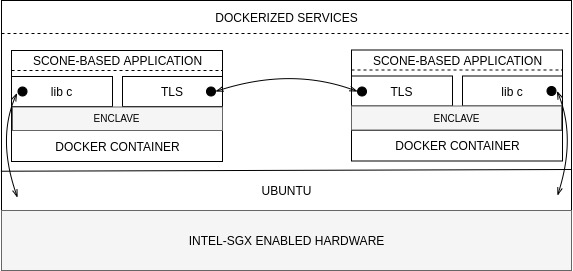
\includegraphics[width=0.7\linewidth]{instanceStack}}
	\caption{Server Component Technology Stack}
	\label{fig:instanceStack}
\end{figure}

1- runs inside docker container with scone image

2- app runs inside enclave

3- has TLS keys and certs upon container creation, allowing it to communicate with other components securely

4- uses small static C library to make system calls directly to the OS, directly from inside the enclave



\subsection{Client-based benchmarks}

To implement the Client, first we tested our solution directly against the \gls{kvs} instances themselves, in order to get base values for the metrics we intend to study. For that we used redis-benchmark, which comes directly with the installation of Redis itself, therefore its version is induced by the Redis version present on the machine.

However, since our solution was designed with a customized entry point API (our Proxy component) which redirects client requests to the Redis \gls{kvs} instances, we were unable to find a way of setting redis-benchmark to make requests to the Proxy. 
Thus, in order to perform a experimental evaluation over the entire TREDIS solution, we opted to used Jmeter\footnote{https://jmeter.apache.org/} version 5.3 as a way to reach our Proxy endpoint, thus benchmarking the behavior of our solution without needing to exclude any component. Also, by being designed by a different organization than the provider of the \gls{kvs} we are studying, it gives an extra level of guarantee in our results, just in case.

With the clients defined as above, we were able to evaluate our system as we intended. 
We made simple \gls{crud} operations to the in-memory Redis \gls{kvs} instances running inside the TREDIS solution, either through the Proxy or directly to Redis instances, along with some other specific tests that we will detail later in this thesis, in order to analyze performance levels, scalability capabilities, resource usage, and other metrics we found a necessity to evaluate.


\section{Tradeoffs on the implementation options}
Discutir overheads daquilo que usámos (openSSL issue, redis monolitico ou não, etc)

- (faz sentido outra vez? igual ao cap 3.4)

\section{Summary}



resumo do modelo de sistema que implementamos, as tecnologias em resumo e essas cenas

TODO - falar daquilo de como sabemos se as cenas estão mesmo a correr na enclave (e apontar po site do scone onde mostram o programa que ve isso)

From SCONE: 
HOW CAN I ENFORCE/VERIFY THAT A SERVICE/PROGRAM RUNS INSIDE OF AN ENCLAVE?
You need to attest that your program runs inside of an enclave. SCONE supports transparent attestation with the help of CAS.

On the application level, one often does not want to perform an explicit attestation but an implicit attestation with the help of TLS to reduce/eliminate the amount of reengineering that is needed. The idea is that a service can only provide the correct TLS certificate if it runs inside an enclave. To do so, one would give the enclave an encrypted TLS private key in the file system (can be generate by Scone CAS if this is requested) and the enclave gets only access to the encryption key after a successful attestation. The decryption of the TLS private key is done transparently by SCONE.


% \lipsum[1-100]
% \lipsum[1-700]
% \lipsum[1-700]
% \lipsum[1-700]
% \lipsum[1-700]
% \lipsum[1-700]
% \lipsum[1-700]
% \lipsum[1-700]
% \lipsum[1-700]
